\documentclass[10.5pt]{beamer}
\usetheme{Madrid}
\usecolortheme{seahorse}
\usepackage{xcolor}
\usepackage[utf8]{inputenc}
\usepackage[spanish]{babel}
\usepackage{amsmath}
\usepackage{amsfonts}
\usepackage{amssymb}
\usepackage{graphicx}
\usepackage{ragged2e}
\usepackage{hyperref}
\setbeamertemplate{navigation symbols}{} 
\author[Kevin García - Alejandro Vargas]{Kevin García 1533173 \newline Alejandro Vargas 1525953}
\title[Anteproyecto]{Diseño y validación de muestreo de cítricos para detección de enfermedades en viveros del Valle del Cauca}


\newcommand\Wider[2][1em]{%
\makebox[\linewidth][c]{%
  \begin{minipage}{\dimexpr\textwidth+#1\relax}
  \raggedright#2
  \end{minipage}%
  }%
}


%\setbeamercovered{transparent} 
%\setbeamertemplate{navigation symbols}{} 
%\logo{} 
%\institute{} 
%\date{} 
%\subject{} 
\begin{document}
\justify
\begin{frame}
\frametitle{Titulo y proyecto}
\begin{block}{Titulo del trabajo}
\justifying
Diseño y validación de muestreo de cítricos para detección de enfermedades en viveros del Valle del Cauca
\end{block}

\begin{block}{Información del proyecto}
\justifying
Entidad encargada: AGROSAVIA (Corpoica)
~\\La Corporación Colombiana de Investigación Agropecuaria, Corpoica, es una entidad pública descentralizada de participación mixta sin ánimo de lucro, de carácter científico y técnico, cuyo objeto es desarrollar y ejecutar actividades de investigación, tecnología y transferir procesos de innovación tecnológica al sector agropecuario.
~\\Personal a cargo:
\begin{itemize}
\item[-]Nubia Murcia Riaño (Investigador Ph.D.)
\item[-]Mauricio Fernando Martínez (Investigador Máster)
\item[-]Elizabeth Narvaez Toro (Líder de Seguimiento y Evaluación)
\end{itemize}
\end{block}
\end{frame}

\begin{frame}
\frametitle{Problema}
\begin{block}{Problema contextual}
\justifying
~\\Existen diversas enfermedades en los cítricos transmitidas principalmente por injertación, vectores (organismos o insectos), y uso de herramienta, las cuales son muy dañinas para este cultivo, entre ellas, el virus de la tristeza, HLB, Leprosis y Exocortis. Estas debilitan el árbol, generando producciones escasas, y en casos avanzados puede llegar a matar el árbol. El inconveniente es que estas enfermedades son asintomáticas en edades tempranas de la planta, es decir, no podemos diferenciar a simple vista una planta infectada con una no infectada. Al sembrar una planta con alguna de estas infecciones desde el comienzo, se perderá mucho dinero invirtiendo en su mantenimiento, por lo cuál se necesita asegurar o garantizar que las plantas que van a ser sembradas y entregadas estén limpias de estas enfermedades, logrando de esta manera la producción de material certificado.
\end{block}
\end{frame}

\begin{frame}
\frametitle{Justificación}
\begin{block}{Problema estadístico}
\begin{itemize}
\justifying
\item ¿Es posible diseñar un plan de muestreo adecuado y asequible que permita la detección temprana de estas enfermedades en los cítricos?
\item ¿Es posible estimar la cantidad de plantas infectadas en los lotes a partir del plan de muestreo diseñado?
\end{itemize}
\end{block}
\begin{block}{Justificación}
\justifying
La agricultura siempre será de gran importancia para el desarrollo de un país, de aquí que la industria de los cítricos requiera normas claras en cuanto a la producción evitando un posible desabastecimiento del producto por una epidemia en plantas de cítricos. Nuestro rol como estadísticos es de vital importancia para lograr verificar con una certeza alta que la producción esté libre de cualquier plaga y mitigar en gran medida posibles pérdidas en toda la industria por lotes infectados, logrando también que tanto consumidores como productores se vean beneficiados.
\end{block}
\end{frame}

\begin{frame}
\frametitle{Objetivos propuestos}
\begin{block}{Objetivo general}
Diseñar y validar un plan de muestreo para aceptación y rechazo de lotes de cítricos en viveros del Valle del Cauca que permita estimar la cantidad de plantas infectadas con el virus de la tristeza en el lote.
\end{block}
\begin{block}{Objetivos específicos}
\begin{itemize}
\justifying
\item[-]Proponer y diseñar diferentes tipos de muestreo tipo aceptación/rechazo para lotes de cítricos en viveros del Valle del Cauca.
\item[-]Validar los diseños muéstrales por medio de simulación teniendo en cuenta confianza y costo del muestreo.
\item[-]Estimar la cantidad de plantas infectadas con el virus de la tristeza.
\end{itemize}
\end{block}
\end{frame}

\begin{frame}
\frametitle{Antecedentes}
\begin{block}{Antecedentes contextuales}
\begin{itemize}
\justifying
\item[1.]Epidemiología de Plum pox virus y citrus tristeza virus en bloques de plantas de vivero. Métodos de control.(2010)\cite{AC1}
\item[2.]Enfermedades causadas por Phytophthora en viveros de plantas ornamentales.(2012)\cite{AC2}
\item[3.]Phytophthora community structure analyses in Oregon nurseries inform systems approaches to disease management.(2014)\cite{AC3}
\item[4.]El Virus de la Tristeza de los Citricos (CTV) en Plantaciones Comerciales y Viveros de la República Dominicana.(2008)\cite{AC4}
\item[5.]Ocurrencia de Huanglongbing (Candidatus Liberibacter asiaticus) y su vector [Diaphorina citri Kuwayama (Hemiptera: Liviidae)] en viveros de cítricos de Masaya.(2018)\cite{AC5}
\end{itemize}
\end{block}
\end{frame}

\begin{frame}
\frametitle{Antecedentes}
\begin{block}{Antecedentes estadísticos}
\begin{itemize}
\justifying
\item[1.]Monitorización del cumplimiento del protocolo de mantenimiento de la cateterización venosa mediante el método LQAS.(2004)\cite{AE1}
\item[2.]Using lot quality assurance sampling to improve immunization coverage in Bangladesh.(2001)\cite{AE2}
\item[3.]Evaluación, mejora y monitorización de la adecuación de ingreso y estancia en Medicina Interna con el muestreo de aceptación de lotes.(2000)\cite{AE3}
\item[4.]Field trial of applicability of lot quality assurance sampling survey method for rapid assessment of prevalence of active tracoma.(2003)\cite{AE4}
\end{itemize}
\end{block}
\end{frame}

\begin{frame}
\frametitle{Marco Teórico}
\begin{block}{Marco conceptual}
\begin{columns}
\column{.15\textwidth}
\begin{itemize}
\item Vivero
\item Lote
\end{itemize}
\column{.20\textwidth}
\begin{itemize}
\item Plaga
\item Prueba
\end{itemize}
\column{.40\textwidth}
\begin{itemize}
\item Virus de la tristeza
\item Huanglongbing(HLB)
\end{itemize}
\column{.25\textwidth}
\begin{itemize}
\item Leprosis
\item Exocortis
\end{itemize}
\end{columns}
\end{block}
\begin{block}{Marco Estadístico}
\begin{columns}
\column{.45\textwidth}
\begin{itemize}
\item Muestreo
\item Muestreo probabilístico
\item Muestreo Aleatorio Simple (MAS)
\item Muestreo sistemático
\item Muestreo estratificado
\item Muestreo secuencial
\item Muestreo por conglomerados
\end{itemize}
\column{.45\textwidth}
\begin{itemize}
\item Muestreo no probabilístico
\item Muestreo de conveniencia
\item Muestreo arbitrario
\item Muestreo selectivo o dirigido
\item Muestreo de aceptación
\item Muestreo Hipergeométrico
\item Muestreo Binomial
\item Muestreo Poisson
\end{itemize}
\end{columns}
\end{block}
\end{frame}

\begin{frame}
\frametitle{Metodología}
\begin{block}{Propuesta}
\begin{itemize}
\item Definición del caso
\item Criterio de aceptación/rechazo
\item Enfermedades (asintomáticas – no asintomáticas)
\item Tipos de vivero (con regulaciones – sin regulaciones)
\item Tipo de muestreo
\item Simulación
\item Análisis y validación del muestreo
\end{itemize}
\end{block}
\end{frame}

\begin{frame}
\frametitle{Cronograma}
\begin{figure}[!h]
        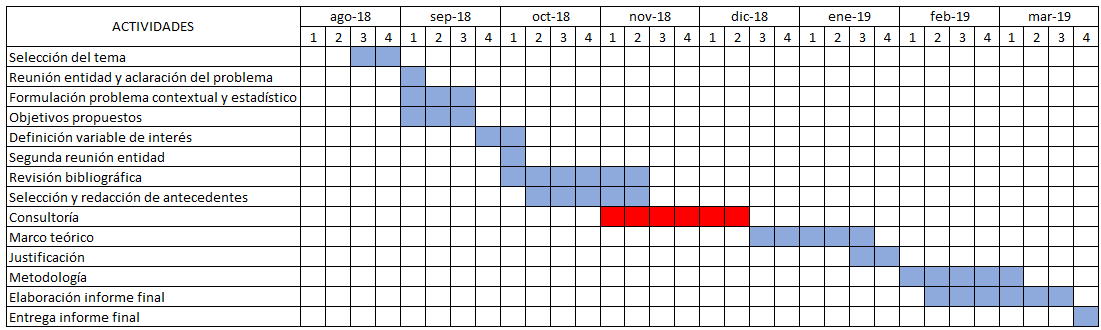
\includegraphics[width=12cm]{IMAGENES/Cron.png}
        \label{figura1}
\end{figure}
\end{frame}

\bibliographystyle{plain}
  \bibliography{references}
\end{document}